\begin{section_4}
\subsection{Описание}
\text{Магнитный фрактал — это концепция, описывающая структуру магнитных полей как фрактальную, то есть обладающую свойством самоподобия на разных масштабах. Исторически фрактальные магнитные поля исследовались в научных работах, например, у Эпштейна и Миллера, которые создали фрактальные магнитные поля в искусственных материалах, обнаружив, что форма магнитного поля в таких материалах не укладывается в традиционные трехмерные модели, а характеризуется дробной размерностью (около 0,8-1,6 мерности)\\}
    
\Lower\[\textbf{z_{n+1} = \left[ \frac{z_n^3 + 3(c-1)z_n + (c-1)(c-2)}{3z_n^2 + 3(c-2)z_n + (c-1)(c-2)} \right]^2}\]

\subsection{Код}
\begin{lstlisting}[language=Python]
import numpy as np
import matplotlib.pyplot as plt
import matplotlib.colors as clr
from itertools import cycle
import os

def magnet_fractal(pmin, pmax, qmin, qmax, ppoints=1000, qpoints=1000,
                  max_iterations=300, infinity_border=40):
    image = np.zeros((ppoints, qpoints))
    p, q = np.mgrid[pmin:pmax:(ppoints*1j), qmin:qmax:(qpoints*1j)]
    c = p + 1j*q
    z = np.zeros_like(c)
    mask = np.ones_like(c, dtype=bool)
    for k in range(1, max_iterations+1):
        with np.errstate(divide='ignore', invalid='ignore'):
            numerator = z**3 + 3*(c-1)*z + (c-1)*(c-2)
            denominator = 3*z**2 + 3*(c-2)*z + (c-1)*(c-2) + 1
            valid = denominator != 0
            # Изменяем только те точки, где делитель не ноль
            z_next = np.where(valid, (numerator/denominator)**2, z)
            z = np.where(valid, z_next, z)
        escape = (np.abs(z) > infinity_border) & mask
        image[escape] = k
        mask[escape] = False
        if not np.any(mask):  # Все вышли за границу
            break
    image[image == 0] = max_iterations
    return -image.T

def make_colormap():
    colorpoints = [
        (1 - (1 - q)**4, c)
        for q, c in zip(
            np.linspace(0, 1, 20),
            cycle(['#ffff88', '#000000', '#ffaa00'])
        )
    ]
    return clr.LinearSegmentedColormap.from_list('mycmap', colorpoints, N=2048)

def render(image, bounds, cmap, filename):
    pmin, pmax, qmin, qmax = bounds
    fig, ax = plt.subplots(figsize=(8, 8))
    ax.imshow(image, extent=(pmin, pmax, qmin, qmax), cmap=cmap, interpolation='none')
    ax.set_title(f"Magnet Fractal 2\nRe∈[{pmin:.2f},{pmax:.2f}] Im∈[{qmin:.2f},{qmax:.2f}]",
                 color='white', fontsize=10)
    ax.set_xticks([]); ax.set_yticks([])
    ax.set_facecolor('black')
    plt.tight_layout()
    os.makedirs("tfkp", exist_ok=True)
    plt.savefig(os.path.join("tfkp", filename), dpi=300, bbox_inches='tight', facecolor='black')
    plt.close(fig)
    print(f"Сохранено: tfkp/{filename}")

if __name__ == "__main__":
    cmap = make_colormap()
    full_bounds = (0.75, 1, 1.25, 1.5)
    image = magnet_fractal(*full_bounds, 1000, 1000, max_iterations=300)
    render(image, full_bounds, cmap, "magnet4_full.png")

\end{lstlisting}
\subsection{Картинки}
\begin{figure}
    \centering
    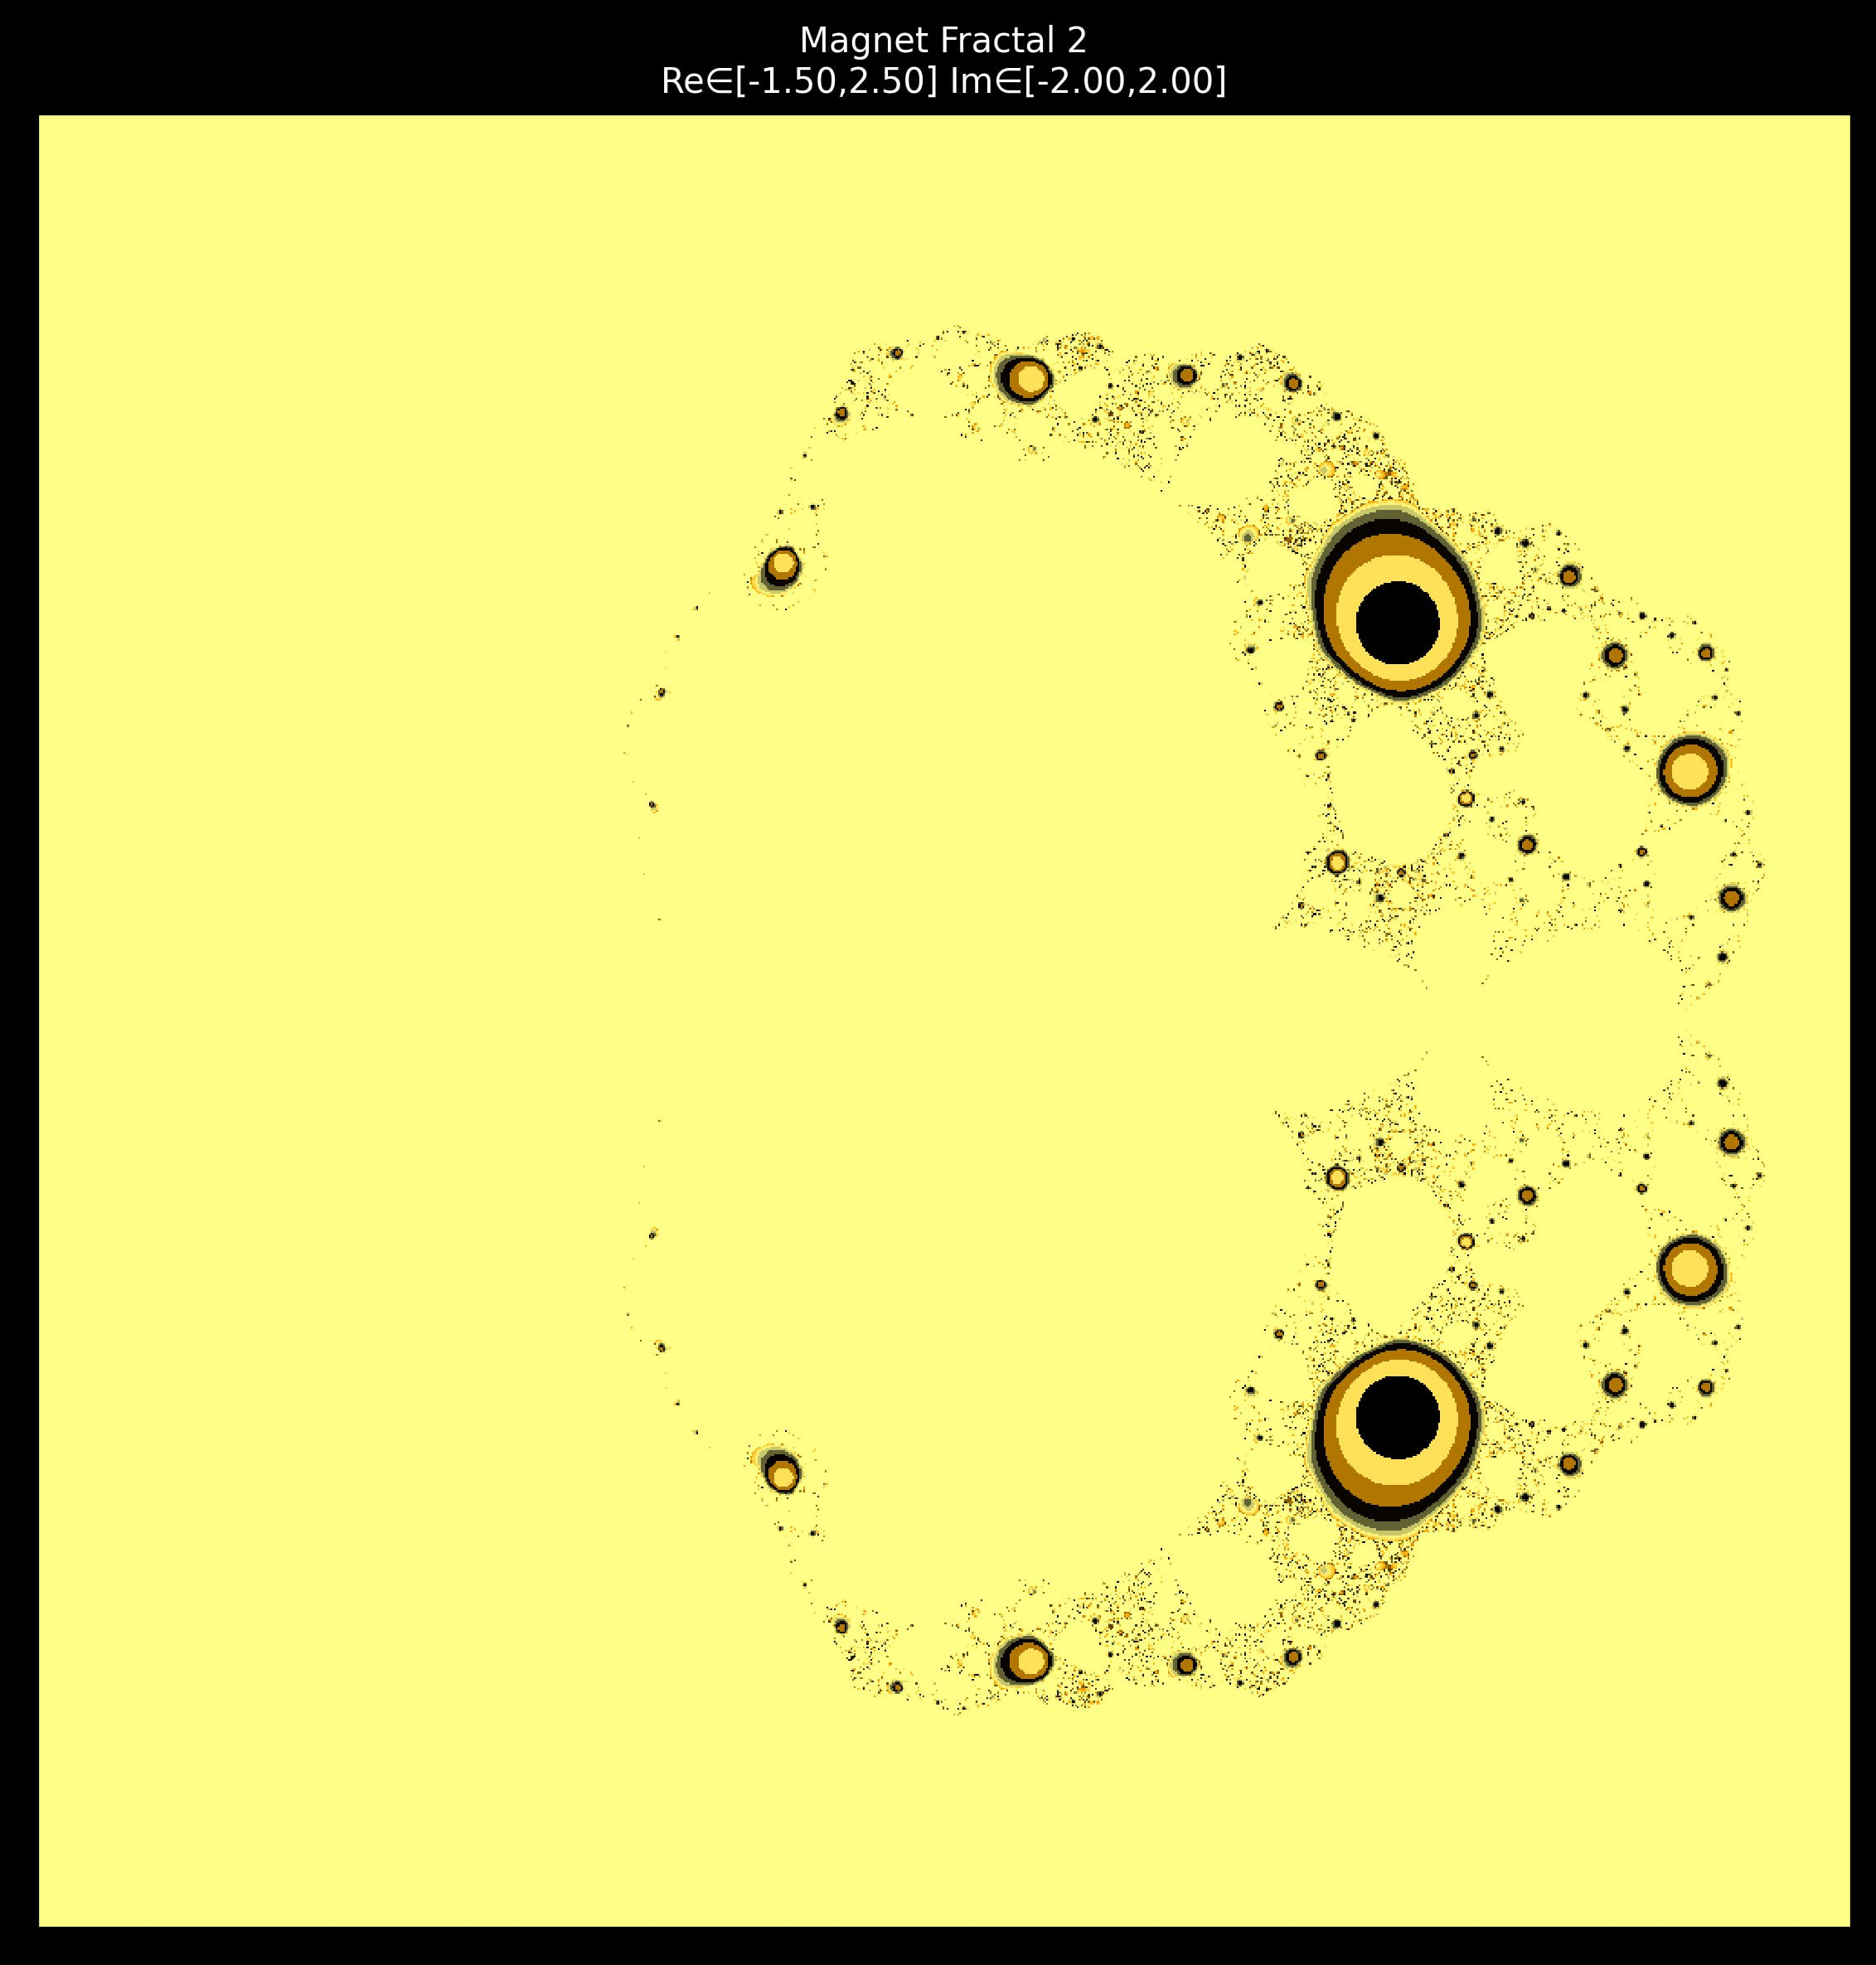
\includegraphics[width=1\linewidth]{photo/ddddd.png}
    \label{fig:placeholder}
\end{figure}
\begin{figure}
    \centering
    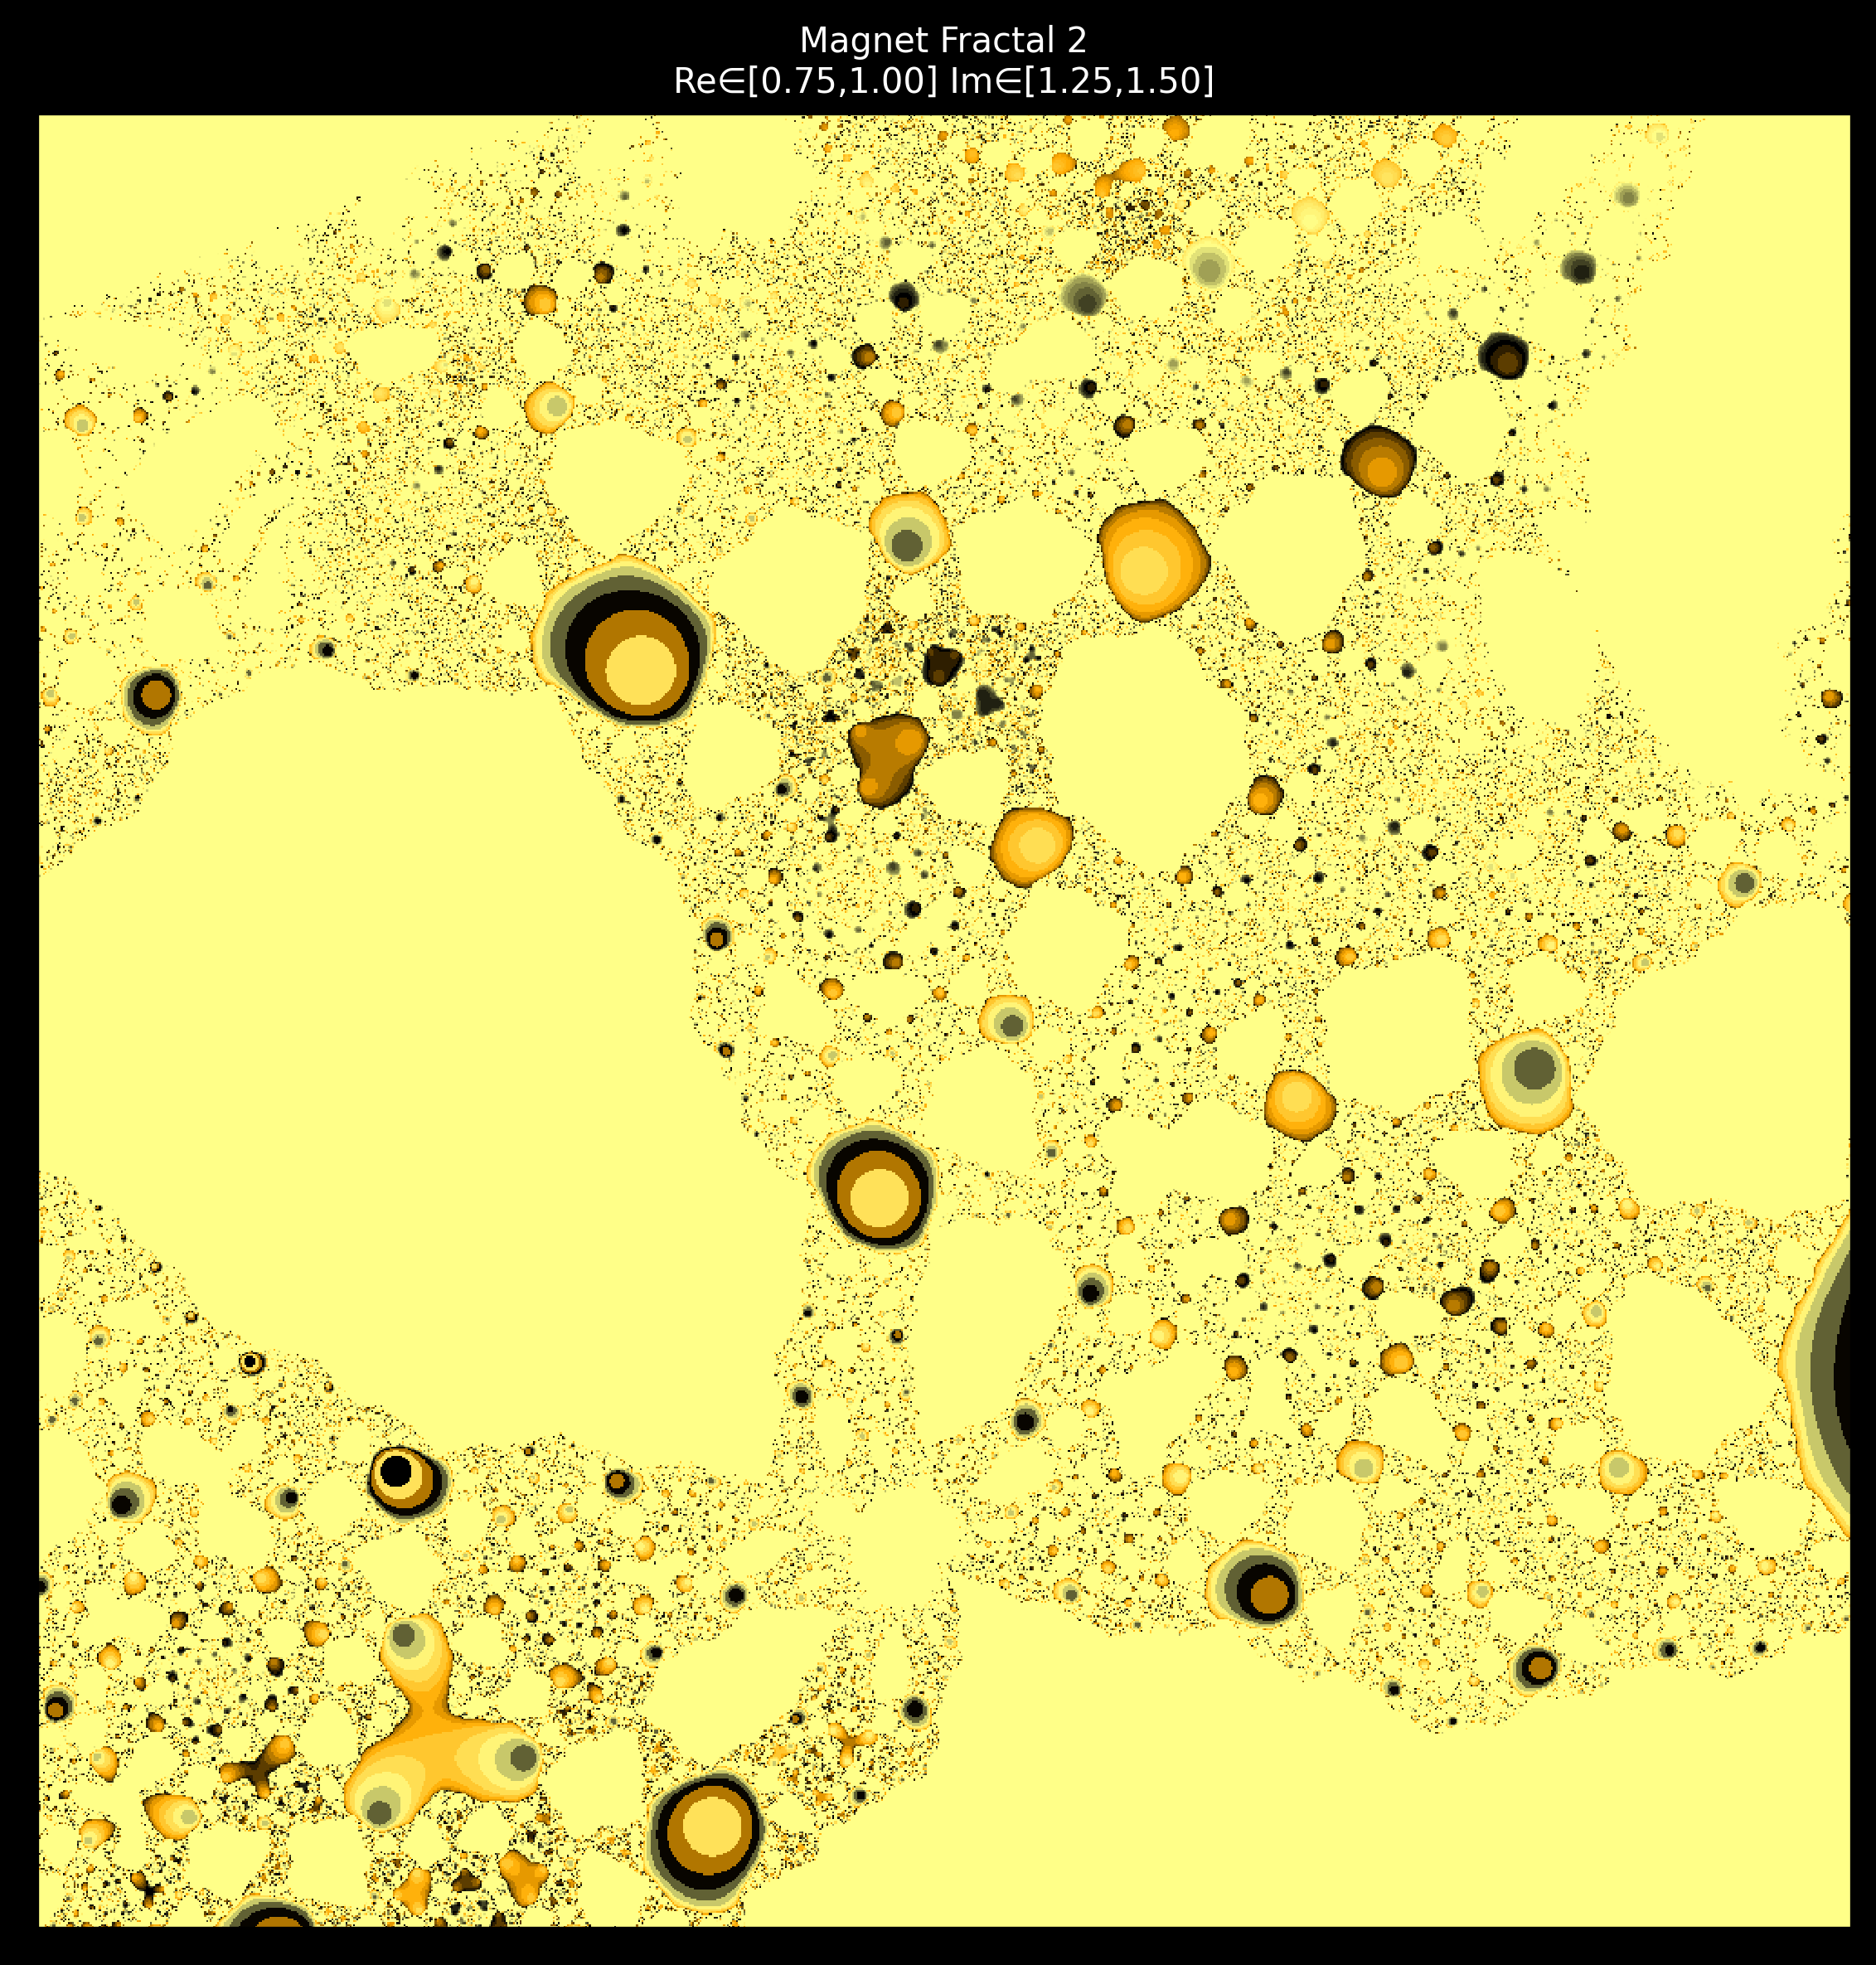
\includegraphics[width=1\linewidth]{photo/magnet4_full1.png}
    \label{fig:placeholder}
\end{figure}
\begin{figure}
    \centering
    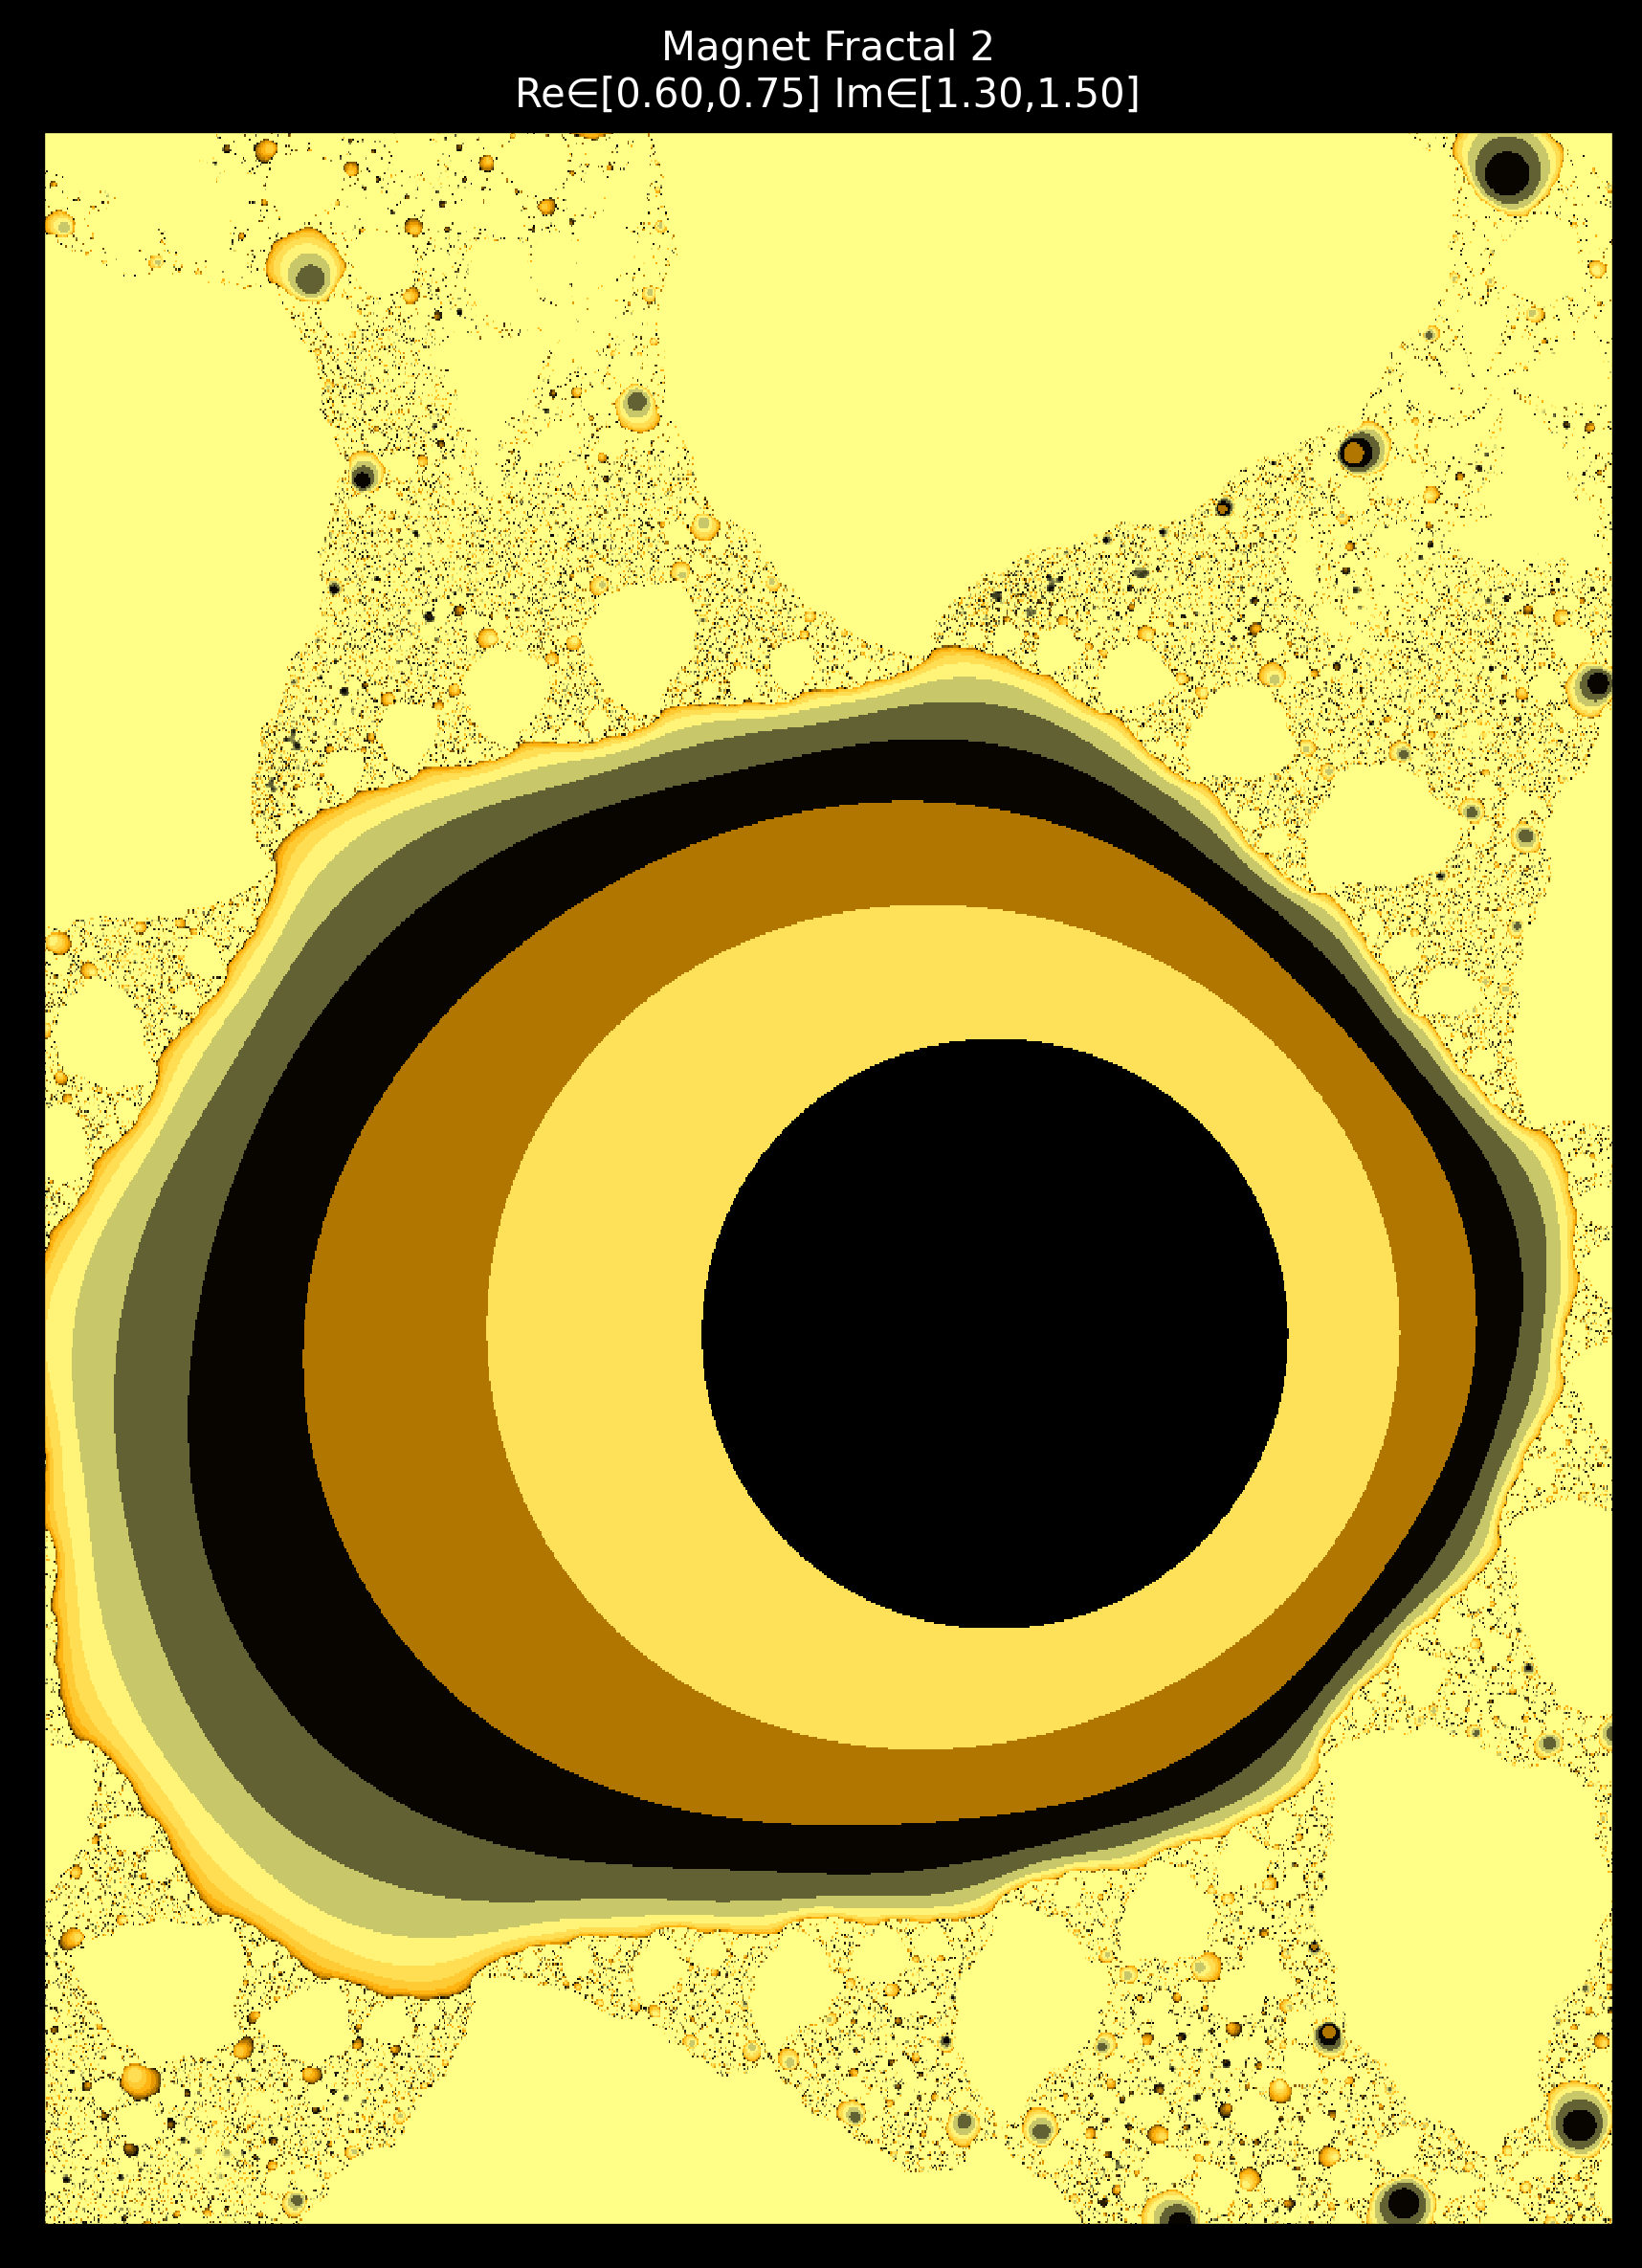
\includegraphics[width=1\linewidth]{photo/magnet4_full.png}
    \label{fig:placeholder}
\end{figure}
\begin{figure}
    \centering
    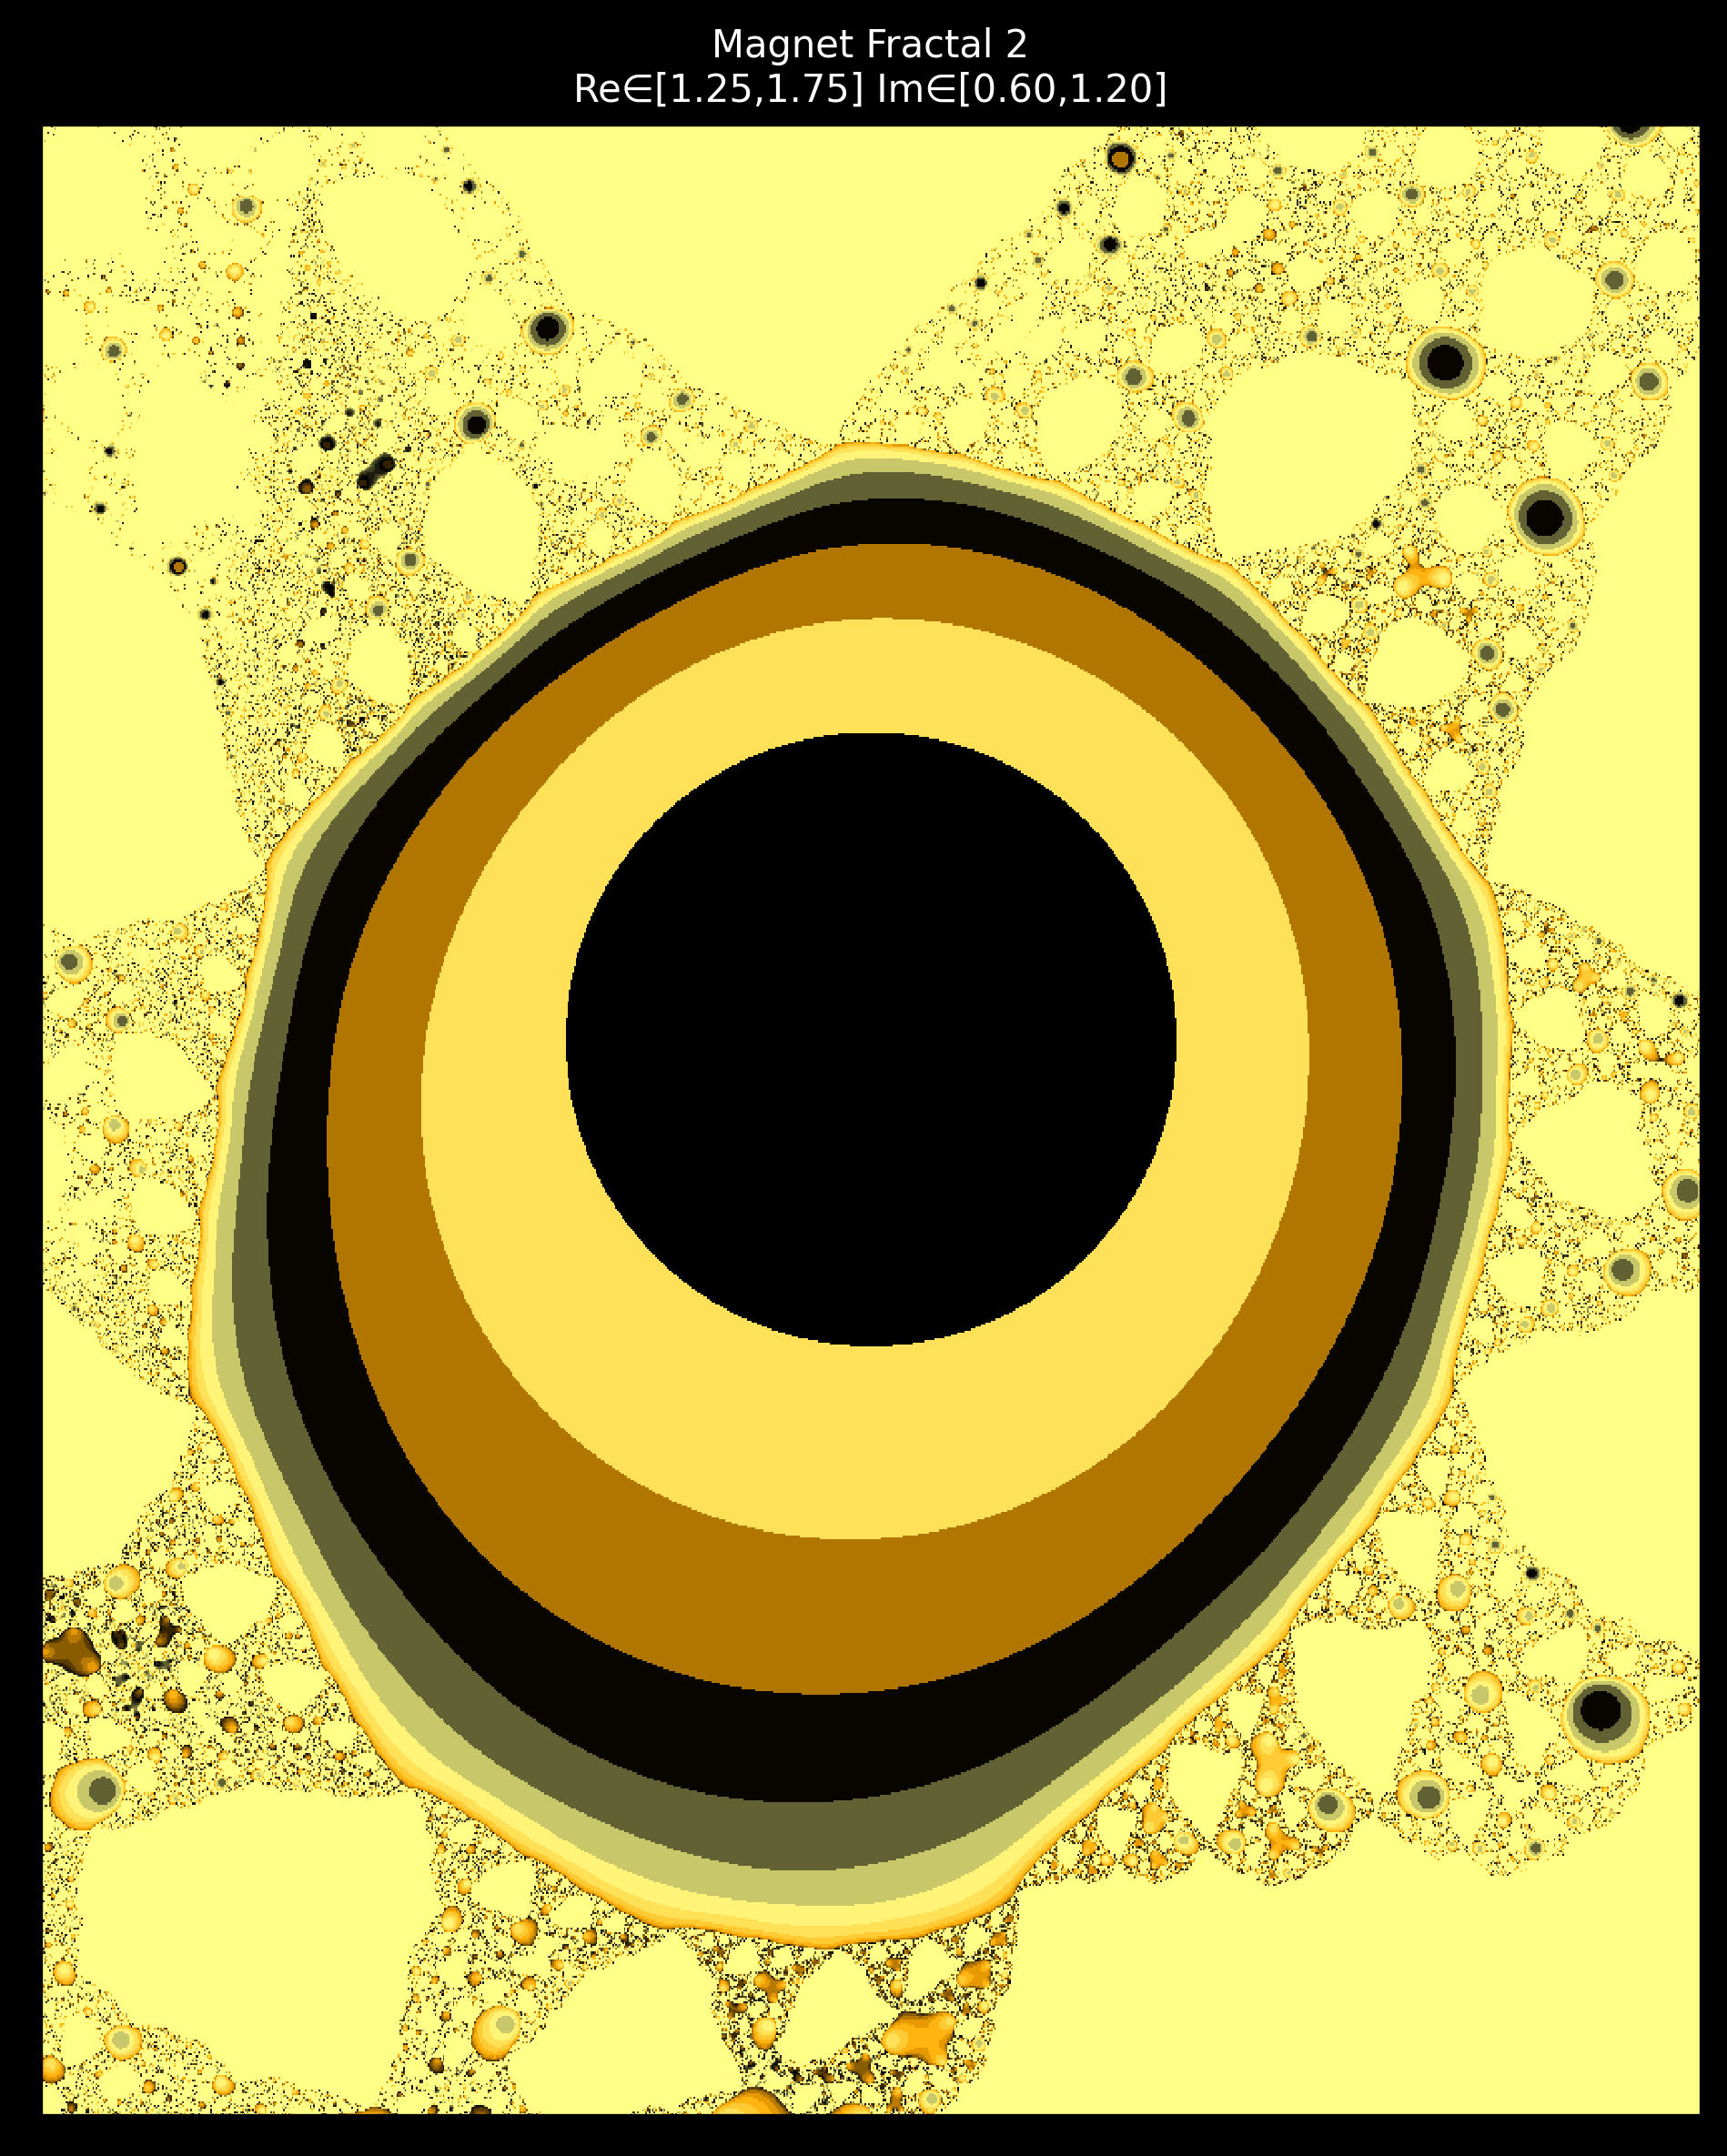
\includegraphics[width=1\linewidth]{photo/magnet3_full.png}
    \label{fig:placeholder}
\end{figure}
\end{section_4}